Direct imaging of exoplanets allows for demographic studies of wide-separation giant planets and for analysis of these planets' atmospheres through spectra and photometry \rev{(e.g. \citealt{2019AJ....158...13N, 2021A&A...651A..72V})}. Each direct imaging detection allows for detailed characterization of the companion \rev{(e.g. \citealt{2008Sci...322.1348M, 2010Natur.468.1080M, 2009A&A...506..927L, 2015Sci...350...64M, 2024Natur.633..789M})}. While wide-separation giant planets have relatively low occurrence rates \rev{(e.g. \citealt{2019AJ....158...13N, 2021A&A...651A..72V})}, additional companions can be identified from astrometric accelerations of their host stars \rev{(e.g. \citealt{2021ApJS..254...42B})}. A targeted survey informed by astrometric accelerations, radial velocities, and stellar ages can complement previous blind surveys by increasing the number of directly imaged substellar companions. Planets detected via astrometry have the added benefit of measurable dynamical masses making them key benchmarks for planet formation and evolution models \rev{(e.g. \citealt{2003IAUS..211..325A, 2021ApJ...920...85M, 2024ApJ...975...59M})}, especially if their ages are known \rev{(e.g. \citealt{2020AJ....159...71N, 2023A&A...672A..94D})}. The mass of a companion can be determined by combining imaging and astrometry, and the companion's age can be measured from observations of the host star. A broader sample of benchmark exoplanets will help constrain planet formation and evolution models.
	
 \textit{Gaia} astrometry is expected to be sensitive to planets between $\sim1-15 \ M_\textrm{Jup}$ with periods between $\sim0.5-10 $ yr around a wide range of stellar host masses \citep{2014ApJ...797...14P}. \textit{Gaia} Data Release 4 (DR4) is scheduled for mid-2026 and is set to include a list of astrometrically detected exoplanets between $\sim1-5$ AU  detected using only \textit{Gaia} \citep{2016A&A...595A...1G}.
 Prior to the release of DR4, substellar companions can be detected by combining positions, parallaxes, and proper motions from the \textit{Hipparcos} Catalog \citep{1997A&A...323L..49P, 1997A&A...323L..61V} and \textit{Gaia} Data Release 3 (DR3) \citep{2023A&A...674A...1G}. Using astrometry the influence of a massive planet on the path of a star can be observed, and longer-period companions can be detected by linking these two missions \rev{(e.g. \citealt{2014ApJ...797...14P, 2021ApJS..254...42B, 2024A&A...684C...2K})}. Velocity is measured as proper motion for stars in both \textit{Hipparcos} (1991.25) and \textit{Gaia} DR3 (2016.0) as well as from the difference between the two catalog positions. An acceleration of the photocenter can be identified from discrepancies between the three velocity vectors. Combined \textit{Hipparcos} and \textit{Gaia} astrometry yield typical acceleration precision as low as $\sim$1\,m\,s$^{-1}$\,yr$^{-1}$ for nearby stars, and is sensitive to longer periods than \textit{Gaia} alone \citep{2021ApJS..254...42B}. 

Several substellar companions have been detected using this method. The $3-7 \ M_\textrm{Jup}$ planet AF Lep b was identified by \rev{the} acceleration of its young host star, a member of the $\sim24$ Myr $\beta$ Pictoris moving group \citep{2015MNRAS.454..593B}, before being detected by direct imaging \citep{2023A&A...672A..94D, 2023A&A...672A..93M, 2023ApJ...950L..19F}. Higher mass substellar companions have been imaged around older accelerating stars including the $13.9-16.1 \ M_\textrm{Jup}$ companion to the $\le 500$ Myr HIP 99770 \citep{2023Sci...380..198C}, the \rev{$\sim28 \ M_ \textrm{Jup}$} companion to the $\sim750$ Myr HIP 21152 \citep{2022ApJ...934L..18K}, and the $\sim31 \ M_\textrm{Jup}$ companion to the \rev{$\lesssim1.5$} Gyr HIP 5319 \citep{2022AJ....164..152S}. Since these accelerations are from astrometric measurements of position and velocity with a limited time baseline, there is a degeneracy between the companion mass and orbital parameters, especially the period. For example, the acceleration of the $\sim500$ Myr HR 1645 appeared to be consistent with a brown dwarf companion on a $\sim100$ yr orbit but was instead shown to be caused by a stellar binary with a $<1$ yr orbit \citep{2019AJ....158..226D}.

Planets cool monotonically over time, with younger, more massive planets being brighter. Given current ground-based direct imaging sensitivity, substellar companions with a contrast ratio brighter than $10^{-6}$ can generally be detected to within $\sim0.5''$ of their host stars \rev{(e.g. \citealt{2014SPIE.9148E..0JM, 2023ASPC..534..799C})}. Depending on the luminosity and distance of the host star, a wide separation ($\sim10-30$ AU) giant planet can be detected around stars younger than a few hundred Myr, and brown dwarfs around stars younger than $\sim1$ Gyr. Thus, measuring accurate ages of host stars and identifying young systems is crucial when selecting high-priority direct imaging targets. We measure the ages of 166 northern hemisphere accelerating stars so that we can identify the youngest systems and prioritize them for direct imaging follow-up.


We use the following methods to derive the ages of our sample stars.
 \begin{enumerate}
     \item  {\bf Ca H and K emission ($R'_{HK}$):} The calcium H and K emission lines are observed as cores within deep absorption lines. The absorption lines form in the optically thick photosphere and the emission cores are generated in the optically thin chromosphere via magnetic heating. Thus, these emission cores trace magnetic activity in stars. As a star spins down with age, its magnetic and chromospheric activity decreases \rev{(e.g. \citealt{1971BAAS....3Q.455S})}. The youngest stars have the fastest rotation and, thus, the strongest magnetic activity, which causes the strongest calcium emission. $R'_{HK}$ is calibrated as an age tracer for F5-K2 stars \rev{(e.g. \citealt{1991ApJ...375..722S, 2008ApJ...687.1264M, 2020ApJ...898...27S})}. 
     
     \item {\bf Lithium:} Throughout the main sequence lifetime of solar-type and lower mass stars, convection transports surface lithium to deeper, hotter layers of the star where it is destroyed via fusion. Lithium depletion is most efficient in low-mass stars that are either fully convective or have thick convective envelopes \citep{1993AJ....105.2299S, 2021A&A...654A.137L, 2010ARA&A..48..581S} making it a useful age tracer for G, K, and M stars. Lithium equivalent width is a powerful age tracer for very young late-type (later than $\sim$K5) stars due to their rapid lithium depletion, but after about $150 $ Myr only equivalent width upper limits can be established for these stars.
     
     \item {\bf Gyrochronology:} Stars later than $\sim$F7 spin down as they age due to angular momentum loss via magnetic braking \citep{1967ApJ...150..551K}. Rotation periods can be measured from flux variations due to star spots rotating on and off the disk of the star. Longer rotation periods correspond to older ages.
     
     \item {\bf Color-Magnitude Diagram Positions:} After reaching the zero-age main sequence, the position of a star on the CMD does not change significantly during the first third of its main sequence lifetime. During the final two-thirds of its main sequence lifetime, the core becomes more helium-rich, increasing the star’s luminosity. This results in detectable movement across the CMD. Age posteriors for these stars can be derived by comparing their photometry to theoretical isochrones \rev{(e.g. \citealt{2013ApJ...776....4N, 2019AJ....158...13N})}. This method is especially powerful for A and F-type stars which have shorter main-sequence lifetimes between $\sim1-5$ Gyr.  

 \end{enumerate}
 
 An approximate schematic of which tracer can produce the most precise age for different stars is shown in Figure \ref{tracers}. Overlap allows for robust age measurements from multiple tracers for some stars. Significant scatter is observed in the age indicators for a given age and mass, which can be quantized to produce a posterior probability distribution on age. The precision of a given age tracer depends on the mass and age of the star. Several tools have been developed to derive age posteriors from these tracers such as \texttt{BAFFLES} \citep{2020ApJ...898...27S}, \texttt{EAGLES} \citep{2023MNRAS.523..802J}, \texttt{stardate} \citep{2019AJ....158..173A}, and \texttt{gyro-interp} \citep{2023ApJ...947L...3B}. We present \rev{median ages and $68\%$ and $95\%$ confidence intervals} for 166 northern hemisphere accelerating stars based on these four age tracers below.
 
 \begin{figure*}[h!]
\centering
 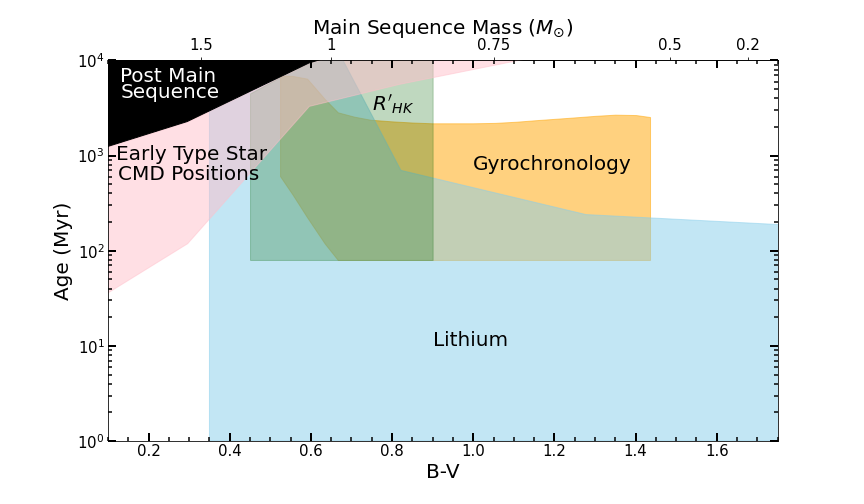
\includegraphics[scale = 0.5]{Tracers_chart.png}
 
 \caption{Age tracers used in this work for young, low-mass stars. This approximate schematic shows which combinations of age and mass are robustly covered by different age tracers. Each shaded region indicates where each tracer is most robust but does not include the regions where limits can be derived from each tracer (e.g. above the blue shaded region lithium is not expected to be detectable, but upper limits on lithium abundance can be used to derive lower limits on the age).}
 \label{tracers}
\end{figure*}




